\chapter{Расширения}
\begin{epigraphs}
\qitem{Гибкость ума может заменить красоту.}{Стендаль}
\end{epigraphs}

\section{Введение}
Один из главных плюсов PostgreSQL это возможность расширения его функционала с помощью расширений. 
В данной статье я затрону только самые интересные и популярные из существующих расширений. 

\section{PostGIS}
\textbf{Лицензия}: Open Source

\textbf{Ссылка}: \href{http://www.postgis.org/}{www.postgis.org}

PostGIS добавляет поддержку для географических объектов в PostgreSQL. По сути PostGIS позволяет использовать PostgreSQL в качестве бэкэнда пространственной базы данных для геоинформационных систем (ГИС), так же, как ESRI SDE или пространственного расширения Oracle. PostGIS соответствует OpenGIS <<Простые особенности. Спецификация для SQL>> и был сертифицирован.
\section{pgSphere}

\href{http://pgsphere.github.io/}{pgSphere} обеспечивает PostgreSQL сферическими типами данных, а также функциями и операторами для работы с ними. Используется для работы с географическими (может использоваться вместо PostGIS) или астрономическими типами данных.

\subsection{Установка и использование}

Для начала инициализируем расширение в базе данных:

\begin{lstlisting}[language=SQL,label=lst:pgsphereinit,caption=Инициализация pgSphere]
# CREATE EXTENSION pg_sphere;
\end{lstlisting}

После этого можем проверить, что расширение функционирует:

\begin{lstlisting}[language=SQL,label=lst:pgsphereex1,caption=Проверка pgSphere]
# SELECT spoly '{ (270d,-10d), (270d,30d), (290d,10d) } ';
                                                          spoly
-------------------------------------------------------------------------------------------------------------------------
 {(4.71238898038469 , -0.174532925199433),(4.71238898038469 , 0.523598775598299),(5.06145483078356 , 0.174532925199433)}
(1 row)
\end{lstlisting}

И работу индексов:

\begin{lstlisting}[language=SQL,label=lst:pgsphereex2,caption=Проверка pgSphere]
# CREATE TABLE test (
#   pos spoint NOT NULL
# );
CREATE TABLE
# CREATE INDEX test_pos_idx ON test USING GIST (pos);
CREATE INDEX
# INSERT INTO test(pos) VALUES ('( 10.1d, -90d)'), ('( 10d 12m 11.3s, -13d 14m)');
INSERT 0 2
# VACUUM ANALYZE test;
VACUUM
# SELECT set_sphere_output('DEG');
 set_sphere_output
-------------------
 SET DEG
(1 row)

# SELECT * FROM test;
                   pos
------------------------------------------
 (10.1d , -90d)
 (10.2031388888889d , -13.2333333333333d)
(2 rows)
# SET enable_seqscan = OFF;
SET
# EXPLAIN SELECT * FROM test WHERE pos = spoint '(10.1d,-90d)';
                                QUERY PLAN
---------------------------------------------------------------------------
 Bitmap Heap Scan on test  (cost=4.16..9.50 rows=2 width=16)
   Recheck Cond: (pos = '(10.1d , -90d)'::spoint)
   ->  Bitmap Index Scan on test_pos_idx  (cost=0.00..4.16 rows=2 width=0)
         Index Cond: (pos = '(10.1d , -90d)'::spoint)
(4 rows)
\end{lstlisting}

\subsection{Заключение}

Более подробно о использовании расширения можно ознакомиться через \href{http://pgsphere.projects.pgfoundry.org/}{официальную документацию}.

\section{HStore}
\textbf{Лицензия}: Open Source

HStore~-- расширение, которое реализует тип данных для хранения ключ/значение в пределах одного значения в PostgreSQL (например, в одном текстовом поле). Это может быть полезно в различных ситуациях, таких как строки с многими атрибутами, которые редко вибираются, или полу-структурированные данные. Ключи и значения являются простыми текстовыми строками.

\subsection{Пример использования}
Для начала активируем расширение:
\begin{lstlisting}[label=lst:hstore1,caption=Активация hstore]
# CREATE EXTENSION hstore;
\end{lstlisting}

Проверим работу расширения:
\begin{lstlisting}[label=lst:hstore2,caption=Проверка hstore]
# SELECT 'a=>1,a=>2'::hstore;
  hstore
----------
 "a"=>"1"
(1 row)
\end{lstlisting}

Как видно на листинге~\ref{lst:hstore2} ключи в hstore уникальны. Создадим таблицу и заполним её данными:

\begin{lstlisting}[label=lst:hstore3,caption=Проверка hstore]
CREATE TABLE products (
   id serial PRIMARY KEY,
   name varchar,
   attributes hstore
);
INSERT INTO products (name, attributes)
VALUES (
  'Geek Love: A Novel',
  'author    => "Katherine Dunn",
  pages     => 368,
  category  => fiction'
),
(
 'Leica M9',
 'manufacturer  => Leica,
  type          => camera,
  megapixels    => 18,
  sensor        => "full-frame 35mm"'
),
( 'MacBook Air 11',
 'manufacturer  => Apple,
  type          => computer,
  ram           => 4GB,
  storage       => 256GB,
  processor     => "1.8 ghz Intel i7 duel core",
  weight        => 2.38lbs'
);
\end{lstlisting}

Теперь можно производить поиск по ключу:
\begin{lstlisting}[label=lst:hstore4,caption=Поиск по ключу]
# SELECT name, attributes->'pages' as page FROM products WHERE attributes ? 'pages';
        name        | page
--------------------+------
 Geek Love: A Novel | 368
(1 row)
\end{lstlisting}

Или по значению ключа:
\begin{lstlisting}[label=lst:hstore5,caption=Поиск по значению ключа]
# SELECT name, attributes->'manufacturer' as manufacturer FROM products WHERE attributes->'type' = 'computer';
       name      | manufacturer
 ----------------+--------------
  MacBook Air 11 | Apple
 (1 row)
\end{lstlisting}

Создание индексов:
\begin{lstlisting}[label=lst:hstore6,caption=Индексы]
CREATE INDEX products_hstore_index ON products USING GIST (attributes);
CREATE INDEX products_hstore_index ON products USING GIN (attributes);
\end{lstlisting}

Можно также cоздавать индекс на ключ:
\begin{lstlisting}[label=lst:hstore7,caption=Индекс на ключ]
CREATE INDEX product_manufacturer
   ON products ((products.attributes->'manufacturer'));
\end{lstlisting}

\subsection{Заключение}

HStore~--- расширение для удобного и индексируемого хранения слабоструктурированых данных в PostgreSQL.
\section{PLV8}
\textbf{Лицензия}: Open Source

\textbf{Ссылка}: \href{http://code.google.com/p/plv8js/}{code.google.com/p/plv8js}

PLV8 является расширением, которое предоставляет PostgreSQL процедурный язык с движком V8 JavaScript. С помощью этого расширения можно писать в PostgreSQL JavaScript функции, которые можно вызывать из SQL.

\subsection{Скорость работы}

V8\footnote{http://en.wikipedia.org/wiki/V8\_(JavaScript\_engine)} компилирует JavaScript код непосредственно в собственный машинный код и с помощью этого достигается высокая скорость работы. Для примера расмотрим расчет числа Фибоначи. Вот функция написана на plpgsql:

\begin{lstlisting}[label=lst:plv8js1,caption=Фибоначи на plpgsql]
CREATE OR REPLACE FUNCTION
psqlfib(n int) RETURNS int AS $$
 BEGIN
     IF n < 2 THEN
         RETURN n;
     END IF;
     RETURN psqlfib(n-1) + psqlfib(n-2);
 END;
$$ LANGUAGE plpgsql IMMUTABLE STRICT;
\end{lstlisting}

Замерим скорость её работы:

\begin{lstlisting}[label=lst:plv8js2,caption=Скорость расчета числа Фибоначи на plpgsql]
SELECT n, psqlfib(n) FROM generate_series(0,30,5) as n;
 n  | psqlfib 
----+---------
  0 |       0
  5 |       5
 10 |      55
 15 |     610
 20 |    6765
 25 |   75025
 30 |  832040
(7 rows)

Time: 16003,257 ms
\end{lstlisting}

Теперь сделаем тоже самое, но с использованием PLV8:

\begin{lstlisting}[label=lst:plv8js3,caption=Фибоначи на plv8]
CREATE OR REPLACE FUNCTION
fib(n int) RETURNS int as $$

  function fib(n) {
    return n<2 ? n : fib(n-1) + fib(n-2)
  }
  return fib(n)

$$ LANGUAGE plv8 IMMUTABLE STRICT;
\end{lstlisting}

Замерим скорость работы:

\begin{lstlisting}[label=lst:plv8js4,caption=Скорость расчета числа Фибоначи на plv8]
SELECT n, fib(n) FROM generate_series(0,30,5) as n;
 n  |  fib   
----+--------
  0 |      0
  5 |      5
 10 |     55
 15 |    610
 20 |   6765
 25 |  75025
 30 | 832040
(7 rows)

Time: 59,254 ms
\end{lstlisting}

Как видим PLV8 приблизительно в 270 (16003.257/59.254) раз быстрее plpgsql. Можно ускорить работу расчета числа Фибоначи на PLV8 за счет кеширования:

\begin{lstlisting}[label=lst:plv8js5,caption=Фибоначи на plv8]
CREATE OR REPLACE FUNCTION
fib1(n int) RETURNS int as $$
  var memo = {0: 0, 1: 1};
  function fib(n) {
    if(!(n in memo))
      memo[n] = fib(n-1) + fib(n-2)
    return memo[n]
  }
  return fib(n);
$$ LANGUAGE plv8 IMMUTABLE STRICT;
\end{lstlisting}

Замерим скорость работы:

\begin{lstlisting}[label=lst:plv8js6,caption=Скорость расчета числа Фибоначи на plv8]
SELECT n, fib1(n) FROM generate_series(0,30,5) as n;
 n  |  fib1  
----+--------
  0 |      0
  5 |      5
 10 |     55
 15 |    610
 20 |   6765
 25 |  75025
 30 | 832040
(7 rows)

Time: 0,766 ms
\end{lstlisting}

Теперь расчет на PLV8 приблизительно в 20892 (16003.257/0.766) раза быстрее, чем на plpgsql.

\subsection{Использование}

Одно из полезных применение PLV8 является создание из PostgreSQL документоориенторованое хранилище. Для хранения неструктурированных данных можно использовать hstore, но у него есть свои недостатки:

\begin{itemize}
\item нет вложенности
\item все данные (ключ и значение по ключу) это строка
\end{itemize}

Для хранения данных многие документоориентированые базы данных используют JSON (MongoDB, CouchDB, Couchbase и т.д.). Для этого начиная с PostgreSQL 9.2 добавлен тип данных JSON. Такой тип можно добавить для PostgreSQL 9.1 и ниже используя PLV8 и DOMAIN:

\begin{lstlisting}[label=lst:plv8js7,caption=Создание типа JSON]
CREATE OR REPLACE FUNCTION 
valid_json(json text)
RETURNS BOOLEAN AS $$
  try { 
    JSON.parse(json); return true; 
  } catch(e) { 
    return false;
  }
$$ LANGUAGE plv8 IMMUTABLE STRICT;

CREATE DOMAIN json AS TEXT 
CHECK(valid_json(VALUE));
\end{lstlisting}

Функция <<valid\_json>> используется для проверки JSON данных. Пример использования:

\begin{lstlisting}[label=lst:plv8js8,caption=Проверка JSON]
$ INSERT INTO members 
VALUES('not good json');
ERROR:  value for domain json 
violates check constraint "json_check"
$ INSERT INTO members 
VALUES('{"good": "json", "is": true}');
INSERT 0 1
$ select * from members;
	    profile            
------------------------------
  {"good": "json", "is": true}
(1 row)
\end{lstlisting}

Расмотрим пример использования JSON для хранения данных и PLV8 для их поиска. Для начала создадим таблицу и заполним её данными:

\begin{lstlisting}[label=lst:plv8js9,caption=Таблица с JSON полем]
$ CREATE TABLE members ( id SERIAL, profile json );
$ SELECT count(*) FROM members;
  count  
---------
 1000000
(1 row)

Time: 201.109 ms
\end{lstlisting}

В <<profile>> поле мы записали приблизительно такую структуру JSON:

\begin{lstlisting}[label=lst:plv8js10,caption=JSON структура]
{                                  +
  "name": "Litzy Satterfield",     +
  "age": 24,                       +
  "siblings": 2,                   +
  "faculty": false,                +
  "numbers": [                     +
    {                              +
      "type":   "work",            +
      "number": "684.573.3783 x368"+
    },                             +
    {                              +
      "type":   "home",            +
      "number": "625.112.6081"     +
    }                              +
  ]                                +
}
\end{lstlisting}

Теперь создадим функцию для вывода значения по ключу из JSON (в данном случае ожидаем цифру):

\begin{lstlisting}[label=lst:plv8js11,caption=Функция для JSON]
CREATE OR REPLACE FUNCTION get_numeric(json_raw json, key text)
RETURNS numeric AS $$
  var o = JSON.parse(json_raw);
  return o[key];
$$ LANGUAGE plv8 IMMUTABLE STRICT;
\end{lstlisting}

Теперь мы можем произвести поиск по таблице фильтруя по значениям ключей <<age>>, <<siblings>> или другим циферным:

\begin{lstlisting}[label=lst:plv8js12,caption=Поиск по данным JSON]
$ SELECT * FROM members WHERE get_numeric(profile, 'age') = 36;
Time: 9340.142 ms
$ SELECT * FROM members WHERE get_numeric(profile, 'siblings') = 1;
Time: 14320.032 ms
\end{lstlisting}

Поиск работает, но скорость очень маленькая. Чтобы улучшить скорость, нужно создать функциональные индексы:

\begin{lstlisting}[label=lst:plv8js13,caption=Создание индексов]
CREATE INDEX member_age ON members (get_numeric(profile, 'age'));
CREATE INDEX member_siblings ON members (get_numeric(profile, 'siblings'));
\end{lstlisting}

С индексами скорость поиска по JSON станет достаточно высокая:

\begin{lstlisting}[label=lst:plv8js14,caption=Поиск по данным JSON с индексами]
$ SELECT * FROM members WHERE get_numeric(profile, 'age') = 36;
Time: 57.429 ms
$ SELECT * FROM members WHERE get_numeric(profile, 'siblings') = 1;
Time: 65.136 ms
$ SELECT count(*) from members where  get_numeric(profile, 'age') = 26 and get_numeric(profile, 'siblings') = 1;
Time: 106.492 ms
\end{lstlisting}

Получилось отличное документоориентированое хранилище из PostgreSQL.

PLV8 позволяет использовать некоторые JavaScript библиотеки внутри PostgreSQL. Вот пример рендера Mustache\footnote{http://mustache.github.com/} темплейтов:

\begin{lstlisting}[label=lst:plv8js15,caption=Функция для рендера Mustache темплейтов]
CREATE OR REPLACE FUNCTION mustache(template text, view json)
RETURNS text as $$
  // …400 lines of mustache.js…
  return Mustache.render(template, JSON.parse(view))
$$ LANGUAGE plv8 IMMUTABLE STRICT;
\end{lstlisting}

\begin{lstlisting}[label=lst:plv8js16,caption=Рендер темплейтов]
$ SELECT mustache(
  'hello {{#things}}{{.}} {{/things}}:) {{#data}}{{key}}{{/data}}',
  '{"things": ["world", "from", "postgresql"], "data": {"key": "and me"}}'
);
		mustache                
---------------------------------------
  hello world from postgresql :) and me
(1 row)

Time: 0.837 ms
\end{lstlisting}

Этот пример показывает как можно использовать PLV8. В действительности рендерить Mustache в PostgreSQL не лучшая идея.

\subsection{Вывод}

PLV8 расширение предоставляет PostgreSQL процедурный язык с движком V8 JavaScript, с помощью которого можно работать с JavaScript билиотеками, индексировать JSON данные и использовать его как более быстрый язык.
\section{Smlar}
\textbf{Лицензия}: Open Source

\textbf{Ссылка}: \href{http://sigaev.ru/git/gitweb.cgi?p=smlar.git;a=blob;hb=HEAD;f=README}{sigaev.ru}

Поиск похожести в больших базах данных является важным вопросом в настоящее время для таких систем как блоги (похожие статьи), интернет-магазины (похожие продукты), хостинг изображений (похожие изображения, поиск дубликатов изображений) и т.д. PostgreSQL позволяет сделать такой поиск более легким. Прежде всего, необходимо понять, как мы будем вычислять сходство двух объектов.

\subsection{Похожесть}

Любой объект может быть описан как список характеристик. Например, статья в блоге может быть описана тегами, продукт в интернет-магазине может быть описан размером, весом, цветом и т.д. Это означает, что для каждого объекта можно создать цифровую подпись~--- массив чисел, описывающих объект (\href{http://en.wikipedia.org/wiki/Fingerprint}{отпечатки пальцев}, \href{http://en.wikipedia.org/wiki/N-gram}{n-grams}). То есть нужно создать массив из цифр для описания каждого объекта. Что делать дальше?

\subsection{Расчет похожести}

Есть несколько методов вычисления похожести сигнатур объектов. Прежде всего, легенда для расчетов:

\begin{itemize}
  \item $N_a$, $N_b$~--- количество уникальных элементов в массивах;
  \item $N_u$~--- количество уникальных элементов при объединении массивов;
  \item $N_i$~--- количество уникальных элементов при пересечение массивов.
\end{itemize}

Один из простейших расчетов похожести двух объектов - количество уникальных элементов при пересечение массивов делить на количество уникальных элементов в двух массивах:

\begin{equation}
 \label{eq:smlar1}
 S(A,B) = \frac{N_{i}}{(N_{a}+N_{b})}
\end{equation}

или проще

\begin{equation}
 \label{eq:smlar2}
 S(A,B) = \frac{N_{i}}{N_{u}}
\end{equation}

Преимущества:

\begin{itemize}
  \item Легко понять;
  \item Скорость расчета: $N * \log{N}$;
  \item Хорошо работает на похожих и больших $N_a$ и $N_b$.
\end{itemize}

Также похожесть можно рассчитана по \href{http://en.wikipedia.org/wiki/Law\_of\_cosines}{формуле косинусов}:

\begin{equation}
 \label{eq:smlar3}
 S(A,B) = \frac{N_{i}}{\sqrt{N_{a}*N_{b}}}
\end{equation}

Преимущества:

\begin{itemize}
  \item Скорость расчета: $N * \log{N}$;
  \item Отлично работает на больших $N$.
\end{itemize}

Но у обоих этих методов есть общие проблемы:

\begin{itemize}
  \item Если элементов мало, то разброс похожести не велик;
  \item Глобальная статистика: частые элементы ведут к тому, что вес ниже;
  \item Спамеры и недобросовестные пользователи. Один <<залетевший дятел>> разрушит цивилизацию - алгоритм перестанет работать на Вас.
\end{itemize}

Для избежания этих проблем можно воспользоваться \href{http://en.wikipedia.org/wiki/Tf*idf}{TF/IDF метрикой}:

\begin{equation}
 \label{eq:smlar4}
 S(A,B) = \frac{\sum_{i < N_{a}, j < N_{b}, A_{i} = B_{j}}TF_{i} * TF_{j}}{\sqrt{\sum_{i < N_{a}}TF_{i}^{2} * \sum_{j < N_{b}}TF_{j}^{2}}}
\end{equation}

где инвертированный вес элемента в коллекции:

\begin{equation}
 \label{eq:smlar5}
 IDF_{element} = \log{(\frac{N_{objects}}{N_{objects\ with\ element}} + 1)}
\end{equation}

и вес элемента в массиве:

\begin{equation}
 \label{eq:smlar6}
 TF_{element} = IDF_{element} * N_{occurrences}
\end{equation}

Не пугайтесь! Все эти алгоритмы встроены в smlar расширение, учить (или даже глубоко понимать) их не нужно. Главное понимать, что для TF/IDF метрики требуются вспомогательная таблица для хранения данных, по сравнению с другими простыми метриками.

\subsection{Smlar}

Перейдем к практике. Олег Бартунов и Теодор Сигаев разработали PostgreSQL расширение smlar, которое предоставляет несколько методов для расчета похожести массивов (все встроенные типы данных поддерживаются) и оператор для расчета похожести с поддержкой индекса на базе GIST и GIN. Для начала установим это расширение (PostgreSQL уже должен быть установлен):

\begin{lstlisting}[language=Bash,label=lst:smlar1,caption=Установка smlar]
$ git clone git://sigaev.ru/smlar
$ cd smlar
$ USE_PGXS=1 make && make install
\end{lstlisting}

В PostgreSQL 9.2 и выше это расширение должно встать без проблем, для PostgreSQL 9.1 и ниже вам нужно сделать небольшое исправление в исходниках. В файле <<smlar\_guc.c>> в строке 214 сделайте изменение с:

\begin{lstlisting}[label=lst:smlar2,caption=Фикс для 9.1 и ниже]
set_config_option("smlar.threshold", buf, PGC_USERSET, PGC_S_SESSION ,GUC_ACTION_SET, true, 0);
\end{lstlisting}

на (нужно убрать последний аргумент):

\begin{lstlisting}[label=lst:smlar3,caption=Фикс для 9.1 и ниже]
set_config_option("smlar.threshold", buf, PGC_USERSET, PGC_S_SESSION ,GUC_ACTION_SET, true);
\end{lstlisting}

Теперь проверим расширение:

\begin{lstlisting}[language=SQL,label=lst:smlar4,caption=Проверка smlar]
$ psql
psql (9.2.1)
Type "help" for help.

test=# CREATE EXTENSION smlar;
CREATE EXTENSION

test=# SELECT smlar('{1,4,6}'::int[], '{5,4,6}'::int[]);
  smlar
----------
 0.666667
(1 row)

test=# SELECT smlar('{1,4,6}'::int[], '{5,4,6}'::int[], 'N.i / sqrt(N.a * N.b)' );
  smlar
----------
 0.666667
(1 row)
\end{lstlisting}

Расширение установлено успешно, если у Вас такой же вывод в консоли. Методы, которые предоставляет это расширение:

\begin{itemize}
  \item \lstinline!float4 smlar(anyarray, anyarray)!~--- вычисляет похожесть двух массивов. Массивы должны быть одного типа;
  \item \lstinline!float4 smlar(anyarray, anyarray, bool useIntersect)!~--- вычисляет похожесть двух массивы составных типов. Составной тип выглядит следующим образом:

\begin{lstlisting}[label=lst:smlar5,caption=Составной тип]
CREATE TYPE type_name AS (element_name anytype, weight_name float4);
\end{lstlisting}

  \lstinline!useIntersect! параметр для использования пересекающихся элементов в знаменателе;
  \item \lstinline!float4 smlar( anyarray a, anyarray b, text formula )!~--- вычисляет похожесть двух массивов по данной формуле, массивы должны быть того же типа. Доступные переменные в формуле:

    \begin{itemize}
      \item N.i~--- количество общих элементов в обоих массивов (пересечение);
      \item N.a~--- количество уникальных элементов первого массива;
      \item N.b~--- количество уникальных элементов второго массива;
    \end{itemize}

  \item \lstinline!anyarray % anyarray!~--- возвращает истину, если похожесть массивов больше, чем указанный предел. Предел указывается в конфиге PostgreSQL:

\begin{lstlisting}[label=lst:smlar6,caption=Smlar предел]
custom_variable_classes = 'smlar'
smlar.threshold = 0.8 # предел от 0 до 1
\end{lstlisting}

Также в конфиге можно указать дополнительные настройки для smlar:

\begin{lstlisting}[label=lst:smlar7,caption=Smlar настройки]
custom_variable_classes = 'smlar'
smlar.threshold = 0.8 # предел от 0 до 1
smlar.type = 'cosine' # по какой формуле производить расчет похожести: cosine, tfidf, overlap
smlar.stattable = 'stat' # Имя таблицы для хранения статистики при работе по формуле tfidf
\end{lstlisting}

Более подробно можно прочитать в README этого расширения.
\end{itemize}

GiST и GIN индексы поддерживаются для оператора \lstinline!%!.

\subsection{Пример: поиск дубликатов картинок}

Рассмотрим простой пример поиска дубликатов картинок. Алгоритм помогает найти похожие изображения, которые, например, незначительно отличаются (изображение обесцветили, добавили водяные знаки, пропустили через фильтры). Но, поскольку точность мала, то у алгоритма есть и позитивная сторона~--- скорость работы. Как можно определить, что картинки похожи? Самый простой метод~--- сравнивать попиксельно два изображения. Но скорость такой работы будет не велика на больших разрешениях. Тем более, такой метод не учитывает, что могли изменять уровень света, насыщенность и прочие характеристики изображения. Нам нужно создать сигнатуру для картинок в виде массива цифр:

\begin{figure}[ht!]
  \center{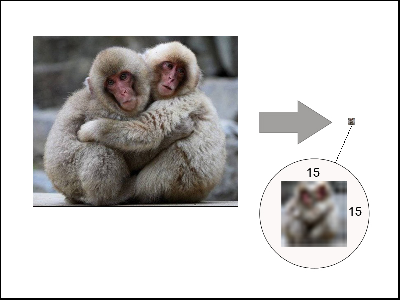
\includegraphics[width=1\textwidth]{smlar1.pdf}}
  \caption{Пиксельная матрица}
  \label{fig:smlar1}
\end{figure}

\begin{itemize}
  \item Создаем пиксельную матрицу к изображению (изменения размера изображения к требуемоему размеру пиксельной матрице), например 15X15 пикселей(Рис.~\ref{fig:smlar1});
  \item Рассчитаем интенсивность каждого пикселя (интенсивность вычисляется по формуле $0.299 * \textup{красный} + 0.587 * \textup{зеленый} + 0.114 * \textup{синий}$). Интенсивность поможет нам находить похожие изображения, не обращая внимание на используемые цвета в них;
  \item Узнаем отношение интенсивности каждого пикселя к среднему значению интенсивности по всей матрице(Рис.~\ref{fig:smlar2});
  \item Генерируем уникальное число для каждой ячейки (отношение интенсивности + координаты ячейки);
  \item Сигнатура для картинки готова.
\end{itemize}

\begin{figure}[ht!]
  \center{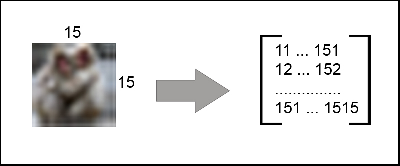
\includegraphics[width=1\textwidth]{smlar2.pdf}}
  \caption{Пиксельная матрица}
  \label{fig:smlar2}
\end{figure}

Создаем таблицу, где будем хранить имя картинки, путь к ней и её сигнатуру:

\begin{lstlisting}[language=SQL,label=lst:smlar8,caption=Таблица для изображений]
CREATE TABLE images (
 id serial PRIMARY KEY,
 name varchar(50),
 img_path varchar(250),
 image_array integer[]
);
\end{lstlisting}

Создадим GIN или GIST индекс:

\begin{lstlisting}[language=SQL,label=lst:smlar9,caption=Создание GIN или GIST индекса]
CREATE INDEX image_array_gin ON images USING GIN(image_array _int4_sml_ops);
CREATE INDEX image_array_gist ON images USING GIST(image_array _int4_sml_ops);
\end{lstlisting}

Теперь можно произвести поиск дубликатов:

\begin{lstlisting}[language=SQL,label=lst:smlar10,caption=Поиск дубликатов]
test=# SELECT count(*) from images;
  count
---------
 1000000
(1 row)

test=# EXPLAIN ANALYZE SELECT count(*) FROM images WHERE images.image_array % '{1010259,1011253,...,2423253,2424252}'::int[];

 Bitmap Heap Scan on images  (cost=286.64..3969.45 rows=986 width=4) (actual time=504.312..2047.533 rows=200000 loops=1)
   Recheck Cond: (image_array % '{1010259,1011253,...,2423253,2424252}'::integer[])
   ->  Bitmap Index Scan on image_array_gist  (cost=0.00..286.39 rows=986 width=0) (actual time=446.109..446.109 rows=200000 loops=1)
         Index Cond: (image_array % '{1010259,1011253,...,2423253,2424252}'::integer[])
 Total runtime: 2152.411 ms
(5 rows)
\end{lstlisting}

где \lstinline!'{1010259,...,2424252}'::int[]!~--- сигнатура изображения, для которой пытаемся найти похожие изображения. С помощью \lstinline!smlar.threshold! управляем \lstinline!%! похожести картинок (при каком проценте они будут попадать в выборку).

Дополнительно можем добавить сортировку по самым похожим изображениям:

\begin{lstlisting}[language=SQL,label=lst:smlar11,caption=Добавляем сортировку по сходству картинок]
test=# EXPLAIN ANALYZE SELECT smlar(images.image_array, '{1010259,...,2424252}'::int[]) as similarity FROM images WHERE images.image_array % '{1010259,1011253, ...,2423253,2424252}'::int[] ORDER BY similarity DESC;


 Sort  (cost=4020.94..4023.41 rows=986 width=924) (actual time=2888.472..2901.977 rows=200000 loops=1)
   Sort Key: (smlar(image_array, '{...,2424252}'::integer[]))
   Sort Method: quicksort  Memory: 15520kB
   ->  Bitmap Heap Scan on images  (cost=286.64..3971.91 rows=986 width=924) (actual time=474.436..2729.638 rows=200000 loops=1)
         Recheck Cond: (image_array % '{...,2424252}'::integer[])
         ->  Bitmap Index Scan on image_array_gist  (cost=0.00..286.39 rows=986 width=0) (actual time=421.140..421.140 rows=200000 loops=1)
               Index Cond: (image_array % '{...,2424252}'::integer[])
 Total runtime: 2912.207 ms
(8 rows)
\end{lstlisting}

Достаточно эффективно для 1 милиона записей(P.S. Мои данные не помещались в память и PostgreSQL читал их с диска, поэтому скорость будет лучше, если у Вас эта таблица будет в памяти или будут быстрые диски).

\subsection{Заключение}

Smlar расширение может быть использовано в системах, где нам нужно искать похожие объекты, такие как: тексты, темы, блоги, товары, изображения, видео, отпечатки пальцев и прочее.
\section{PostPic}

\href{http://drotiro.github.io/postpic/}{PostPic} расширение для PostgreSQL, которое позволяет обрабатывать изображения в базе данных, как PostGIS делает это с пространственными данными. Он добавляет новый типа поля \lstinline!image!, а также несколько функций для обработки изображений (обрезка краев, создание миниатюр, поворот и т.д.) и извлечений его атрибутов (размер, тип, разрешение). Более подробно о возможностях расширения можно ознакомится на \href{https://github.com/drotiro/postpic/wiki/SQL-Functions-Guide}{официальной странице}.

\section{Fuzzystrmatch}
\textbf{Лицензия}: Open Source

Fuzzystrmatch предоставляет несколько функций для определения сходства и расстояния между строками. Функция soundex используется для согласования сходно звучащих имен путем преобразования их в одинаковый код. Функция difference преобразует две строки в soundex код, а затем сообщает количество совпадающих позиций кода. В soundex код состоит из четырех символов, поэтому результат будет от нуля до четырех: 0~--- не совпадают, 4~--- точное совпадение (таким образом, функция названа неверно~--- как название лучше подходит similarity):

\begin{lstlisting}[language=SQL,label=lst:ext_fuzzystrmatch1,caption=soundex]
# CREATE EXTENSION fuzzystrmatch;
CREATE EXTENSION
# SELECT soundex('hello world!');
 soundex
---------
 H464
(1 row)

# SELECT soundex('Anne'), soundex('Ann'), difference('Anne', 'Ann');
 soundex | soundex | difference
---------+---------+------------
 A500    | A500    |          4
(1 row)

# SELECT soundex('Anne'), soundex('Andrew'), difference('Anne', 'Andrew');
 soundex | soundex | difference
---------+---------+------------
 A500    | A536    |          2
(1 row)

# SELECT soundex('Anne'), soundex('Margaret'), difference('Anne', 'Margaret');
 soundex | soundex | difference
---------+---------+------------
 A500    | M626    |          0
(1 row)

# CREATE TABLE s (nm text);
CREATE TABLE
# INSERT INTO s VALUES ('john'), ('joan'), ('wobbly'), ('jack');
INSERT 0 4
# SELECT * FROM s WHERE soundex(nm) = soundex('john');
  nm
------
 john
 joan
(2 rows)

# SELECT * FROM s WHERE difference(s.nm, 'john') > 2;
  nm
------
 john
 joan
 jack
(3 rows)
\end{lstlisting}

Функция levenshtein вычисляет \href{http://en.wikipedia.org/wiki/Levenshtein\_distance}{расстояние Левенштейна} между двумя строками. \lstinline!levenshtein_less_equal! ускоряется функцию levenshtein для маленьких значений расстояния:

\begin{lstlisting}[language=SQL,label=lst:ext_fuzzystrmatch2,caption=levenshtein]
# SELECT levenshtein('GUMBO', 'GAMBOL');
 levenshtein
-------------
           2
(1 row)

# SELECT levenshtein('GUMBO', 'GAMBOL', 2, 1, 1);
 levenshtein
-------------
           3
(1 row)

# SELECT levenshtein_less_equal('extensive', 'exhaustive', 2);
 levenshtein_less_equal
------------------------
                      3
(1 row)

test=# SELECT levenshtein_less_equal('extensive', 'exhaustive', 4);
 levenshtein_less_equal
------------------------
                      4
(1 row)
\end{lstlisting}

Функция metaphone, как и soundex, построена на идее создания кода для строки: две строки, которые будут считатся похожими, будут иметь одинаковые коды. Последним параметром указывается максимальная длина metaphone кода. Функция \lstinline!dmetaphone! вычисляет два <<как звучит>> кода для строки~--- <<первичный>> и <<альтернативный>>:

\begin{lstlisting}[language=SQL,label=lst:ext_fuzzystrmatch3,caption=metaphone]
# SELECT metaphone('GUMBO', 4);
 metaphone
-----------
 KM
(1 row)
# SELECT dmetaphone('postgresql');
 dmetaphone
------------
 PSTK
(1 row)

# SELECT dmetaphone_alt('postgresql');
 dmetaphone_alt
----------------
 PSTK
(1 row)
\end{lstlisting}



\section{Tsearch2}
\textbf{Лицензия}: Open Source

Tsearch2~-- расширение для полнотекстового поиска. Встроен в PostgreSQL начиная с версии 8.3.

\section{OpenFTS}
\textbf{Лицензия}: Open Source

\textbf{Ссылка}: \href{http://openfts.sourceforge.net/}{openfts.sourceforge.net}

OpenFTS (Open Source Full Text Search engine) является продвинутой PostgreSQL поисковой системой, которая обеспечивает 
онлайн индексирования данных и актуальность данных для поиска по базе. Тесная интеграция с базой данных позволяет использовать метаданные, 
чтобы ограничить результаты поиска.

\section{PL/Proxy}
\textbf{Лицензия}: Open Source

\textbf{Ссылка}: \href{http://pgfoundry.org/projects/plproxy/}{pgfoundry.org/projects/plproxy}

PL/Proxy представляет собой прокси-язык для удаленного вызова процедур и партицирования данных между разными базами. 
Подробнее можно почитать в \Sref{sec:plproxy} главе.

\section{Texcaller}
\textbf{Лицензия}: Open Source

\textbf{Ссылка}: \href{http://www.profv.de/texcaller/}{www.profv.de/texcaller}

Texcaller~--- это удобный интерфейс для командной строки TeX, который обрабатывает все виды ошибок. Он написан в простом C, довольно портативный, 
и не имеет внешних зависимостей, кроме TeX. Неверный TeX документ обрабатывается путем простого возвращения NULL, 
а не прерывается с ошибкой. В случае неудачи, а также в случае успеха, дополнительная обработка информации осуществляется через NOTICEs.

\section{Pgmemcache}
\textbf{Лицензия}: Open Source

\textbf{Ссылка}: \href{http://pgfoundry.org/projects/pgmemcache/}{pgfoundry.org/projects/pgmemcache}

Pgmemcache~--- это PostgreSQL API библиотека на основе libmemcached для взаимодействия с memcached. С помощью данной библиотеки 
PostgreSQL может записывать, считывать, искать и удалять данные из memcached. Подробнее можно почитать в \Sref{sec:pgmemcache} главе.

\section{Prefix}
\textbf{Лицензия}: Open Source

\textbf{Ссылка}: \href{http://pgfoundry.org/projects/prefix}{pgfoundry.org/projects/prefix}

Prefix реализует поиск текста по префиксу (prefix @> text). 
Prefix используется в приложениях телефонии, где маршрутизация вызовов и расходы зависят от вызывающего/вызываемого префикса телефонного номера оператора.

\section{Dblink}
\textbf{Лицензия}: Open Source

Dblink~-- расширение, которое позволяет выполнять запросы к удаленным базам данных непосредственно из SQL, не прибегая к помощи внешних скриптов.

\section{Ltree}
\textbf{Лицензия}: Open Source

Ltree~-- расширение, которое позволяет хранить древовидные структуры в виде меток, а также предоставляет широкие возможности поиска по ним. Реализация алгоритма \href{http://en.wikipedia.org/wiki/Materialized\_path}{Materialized Path} (достаточно быстрый как на запись, так и на чтение).

\section{Заключение}
Расширения помогают улучшить работу PostgreSQL в решении специфических проблем. Расширяемость PostgreSQL позволяет создавать собственные расширения, 
или же наоборот, не нагружать СУБД лишним, не требуемым функционалом.